\documentclass{article}

\usepackage[utf8]{inputenc}
\usepackage{url}
\usepackage{fancyhdr}
\usepackage{float}
\usepackage{tikz}
\usetikzlibrary{arrows}
\usetikzlibrary{positioning}
\pagestyle{fancy}

\renewcommand\thepart{\Alph{part}}

\title{Homework Module: A Controller for Swarm Behaviour in Webots}

\lhead{Homework Module \#1}
\rhead{IT3708 - Subsymbolic Methods in AI}

\author{
    Aleksander Burkow \\
    Sigve Sebstian Farstad \\
    Emil Grønnbeck
}

\begin{document}

\maketitle
\thispagestyle{empty}

\abstract{
This report presents a solution for Homework Module \#1 of IT3708, spring 2014 at NTNU.
The purpose of the homework module is to ``understand swarm behaviour by implementing a controller for box pushing task in Webots''.
}

\newpage

\setcounter{page}{1}

\part{The Proposed System}

This is a citation of the assignment ~\cite{assignment}.

\section{Description}


\subsection{Swarm intelligence in nature}



\subsection{Brooks Architecture}
The system we implemented is based on an AI concept called subsumption architecture. Subsumption architecture was first described by Rodney Brooks in the mid 80's. The idea behind subsumption architecture came from insects. Insects though with relatively little computational power, is able to walk, avoid obstacles, and make desicions faster than any robot created. The architecture is divided into layers called: "the levels of competence". Each layer is  independent of each other, where the higher levels are capable of overriding the lower[1]. The highest stimulated behaviour is acted upon [2]

\subsection{Our implementation}
We divided our "levels of competence" into six independent behaviours; Wander, Avoid obstacles, Converge, Retrieve, Realign, and Reposition. The lower levels have a higher priority and are able to override the higher ones.
\begin{figure}[H]
\centering
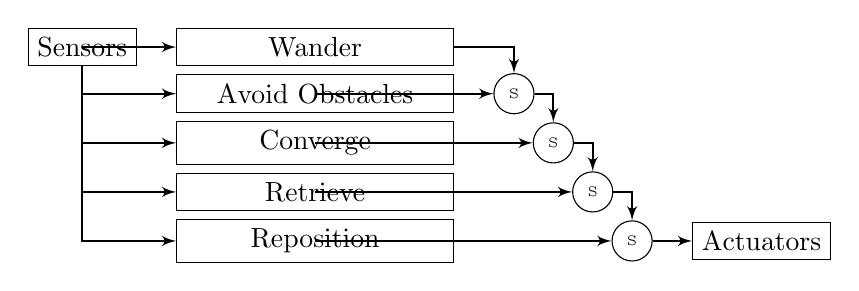
\begin{tikzpicture}

\tikzstyle{behaviour}=[draw, minimum width=10em, right=5mm of sensors]
\tikzstyle{line}=[draw, thick, -latex']
\tikzstyle{subsumption}=[draw, circle]

\node[draw] (sensors) {Sensors};

\node[behaviour] (wander) {Wander};
\node[behaviour, below=1mm of wander] (avoid_obstacles) {Avoid Obstacles};
\node[behaviour, below=1mm of avoid_obstacles] (converge) {Converge};
\node[behaviour, below=1mm of converge] (retrieve) {Retrieve};
\node[behaviour, below=1mm of retrieve] (reposition) {Reposition};

\node[subsumption, right=5mm of avoid_obstacles] (avoid_obstacles_subsumption) {\tiny S};
\node[subsumption, right=10mm of converge] (converge_subsumption) {\tiny S};
\node[subsumption, right=15mm of retrieve] (retrieve_subsumption) {\tiny S};
\node[subsumption, right=20mm of reposition] (reposition_subsumption) {\tiny S};
\node[draw, right=5mm of reposition_subsumption] (actuators) {Actuators};

\path[line] (sensors) |- (wander);
\path[line] (sensors) |- (avoid_obstacles);
\path[line] (sensors) |- (converge);
\path[line] (sensors) |- (retrieve);
\path[line] (sensors) |- (reposition);

\path[line] (avoid_obstacles) |- (avoid_obstacles_subsumption);
\path[line] (converge) |- (converge_subsumption);
\path[line] (retrieve) |- (retrieve_subsumption);
\path[line] (reposition) |- (reposition_subsumption);

\path[line] (wander) -| (avoid_obstacles_subsumption);
\path[line] (avoid_obstacles_subsumption) -| (converge_subsumption);
\path[line] (converge_subsumption) -| (retrieve_subsumption);
\path[line] (retrieve_subsumption) -| (reposition_subsumption);
\path[line] (reposition_subsumption) -- (actuators);

\end{tikzpicture}
\caption{The subsumption architecture of the proposed system.}
\label{figure:subsumption}
\end{figure}


\subsubsection{Wander}
Wander is our default behaviour, it basically tells the robot to run straight forward. It has no stimulus, when no other behaviour is stimulated, the robot acts on this behaviour

\subsubsection{Avoid obstacles}


\subsubsection{Converge}


\subsubsection{Retrieve}

\subsubsection{Realign}

\subsubsection{Reposition}

\section{Simulation Results}

\begin{table}[h!]
\centering
\begin{tabular}{ c | c | p{5cm}}
\hline No & Time & Notes \\ \hline
 1 & 42.56 &  \\ \hline
 2 & 38.21 & \\ \hline
 3 & 33.54 & Close to optimal run \\ \hline
4 & - & Two robots got stuck between the box and the wall. Therefore the robots was not able to finish the objective \\ \hline
5 & 36.35 & \\ \hline
6	& 52.13 & The robots did change pushing direction in the middle of the simulation \\ \hline
7 & 59.81 & \\ \hline
8 & 52.83 & \\ \hline
9 & 3:32.01 &  The robots divided into two groups and pushed from opposite sides \\ \hline
10 & 1:42.84 & The robots divided into two groups and pushed from oppsite sides, though the stagnation got solved earlier than simulation 9 \\
\end{tabular}
\caption{One box problem runs}
\end{table}


\begin{table}
\centering
\begin{tabular}{ l | r}
\hline Number of runs & Avg. Time \\ \hline
9 & ?:??:?? \\
\end{tabular}
\caption{ Average time of One box problem runs}
\end{table}


\subsection{Observed weaknesses}
\part{An Improved System}

\section{Description}
\section{Simulation Results}
\part{A More Advanced Architecture}

\section{Description}
\section{Simulation Results}

\bibliography{reference-library}
\bibliographystyle{plain}

\end{document}
